{\bf Introduction}

\begin{wrapfigure}{l}{0.25\textwidth}
    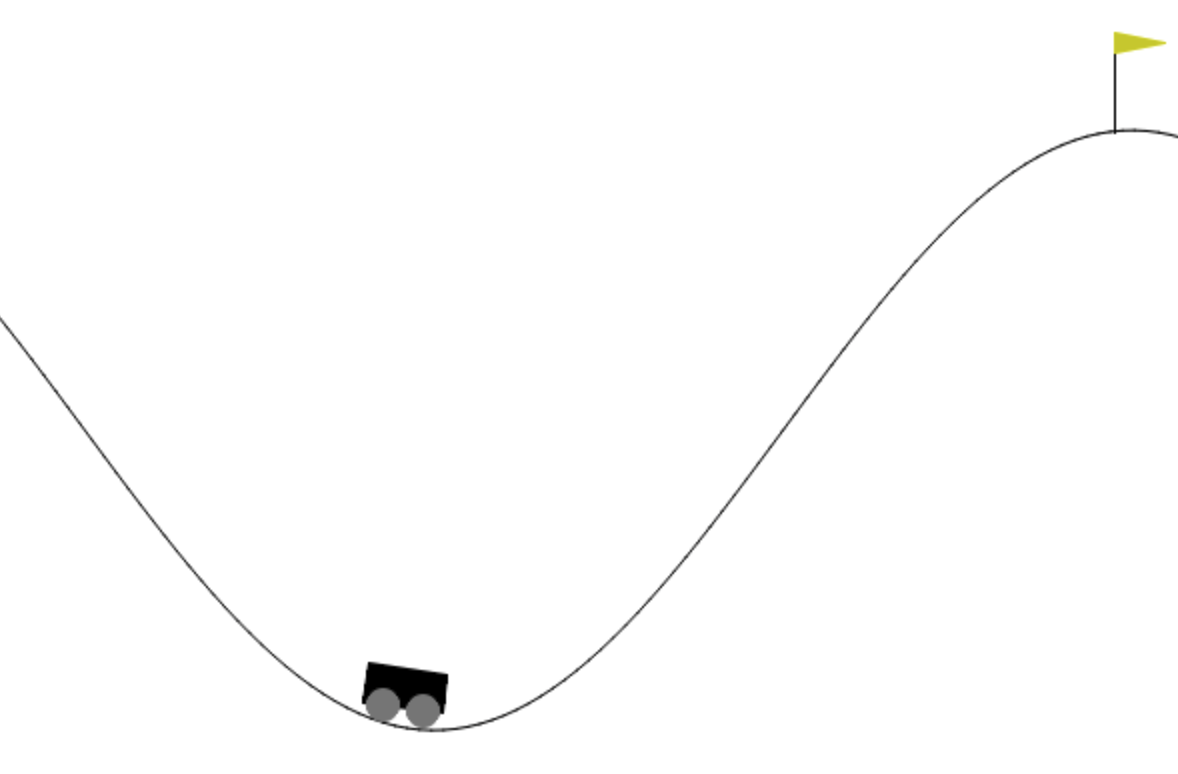
\includegraphics[width=0.9\linewidth]{mountaincar.png} 
    \caption{Mountain Car}
\end{wrapfigure}
    
Markov decision processes (MDPs) can be used to model situations with uncertainty (which is most of the time in the real world). In this assignment, you will implement algorithms to find the optimal policy, even you know the transitions and rewards (value iteration) and when you don't (reinforcement learning). You will use these algorithms on Mountain Car, a classic control environment where the goal is to control a car to go up a mountain.